\documentclass[10pt,a4paper]{article}
\usepackage[margin=20mm]{geometry}
\usepackage{amsmath,amssymb,array,graphicx,hyperref}
\hypersetup{colorlinks=true,urlcolor=blue,linkcolor=blue,pdftitle={Experimental comparison and deformation assessment}}
\newcommand{\rw}[1]{\mathord{#1\mkern2mu\wedge}}
\newcommand{\inertia}{\mathbb I}
\DeclareFontFamily{U}{reportbb}{}
\DeclareFontShape{U}{reportbb}{m}{n}{<-6> bbold5 <6-9> bbold7 <9-> bbold10}{}
\DeclareMathAlphabet{\matrixdigit}{U}{reportbb}{m}{n}
\pdfmapfile{+../scaled-contact-article/fonts/blackboard/bbold.map}
\newcommand{\id}{\matrixdigit{1}}
\setlength{\parindent}{0pt}\setlength{\parskip}{7pt}
\begin{document}
\begin{center}\Large Experimental comparison and deformation assessment\\[4pt]
\normalsize Rigid-body linear and independent angular impulses\\7 October 2026\end{center}
\section*{Experimental comparison and physical scope}

\textbf{We do not yet have a model validated across the real-life datasets.}
This report covers every presently recovered comparison record: 24 glass collisions,
eight oblique ball/surface summaries, 75 rock impacts, and 17 rolling measurements.
These are public experimental records, not invented target states. They are not
124 independently characterized full-state events: some coefficients summarize
overlapping characterization data. Numerical verification and experimental agreement
are separate questions.

Documented parameters remain fixed. Missing parameters are estimated only in small,
explicit calibration models. Same-outcome fitting is not prediction. Every unfavorable
result is retained. The full engine still lacks validated rolling/torsional material
closure and has unresolved rapid irregular-contact cases. No 2x performance gate is
applied; the user removed it.
\begin{center}\footnotesize\setlength{\tabcolsep}{4pt}
\begin{tabular}{llll}
\hline
Comparison & Records & Outcome & Qualification\\\hline
Glass fixed-input comparator & 24 & 0.0367 / 0.0178 m/s RMSE & No independent spin\\
Ball endpoint/moment test & 8 & 4 passive rolling nominal fits & Singleton calibration\\
Shared moment, held-out surface & 8 & RMSE 1.048 to 1.243 rad/m & Worse; rejected\\
Rock sphere-proxy comparator & 50 + 25 & Spin RMSE 12.88 rad/s & Actual shape absent\\
Tennis rolling, held-out speed & 9 + 8 & Constant worse than source curves & Quasirolling only\\
Isolated rolling mechanics & 200 & All pass at three length scales & Synthetic controls\\
\hline\end{tabular}\end{center}
The strongest result is a consistent impulse/momentum framework including an
independent angular impulse. That framework alone does not specify authentic contact
forces. Energy-passive estimates can still predict poorly; this is demonstrated here.
No comparison in this report establishes full 3D actual-shape validation with measured
signed angular-velocity vectors and independently measured inertia tensors.

\newpage
\section*{Mechanics used and physical checks}

The notation retains the user's combined variables and inertia symbol:
\[
 \mathbf V=\begin{bmatrix}\mathbf v\\\ell\boldsymbol\omega\end{bmatrix},\quad
 \mathbf P=\begin{bmatrix}\mathbf p\\\mathbf L/\ell\end{bmatrix},\quad
 \Delta\mathbf P_c=\begin{bmatrix}\delta\mathbf p\\\delta\mathbf L/\ell\end{bmatrix}.
\]
The full angular update is
\[
 \Delta\mathbf L_k=\rw{\mathbf r_k}\,\delta\mathbf p+\delta\mathbf L.
\]
The independent couple is not the lever-arm moment counted twice. In the ball
calculations the input has no spin and the plane fixes the onset axis of generated
spin. This is a declared planar onset branch, not a recovered general mixed-spin law.
All scalar directional components remain in the recorded output.

Keep $\hat{\mathbf t}$ along full relative contact velocity. When it contains normal
approach, the source's normal/tangential friction must be transformed through the
direction map. With $c=\hat{\mathbf n}^{\mathsf T}\hat{\mathbf t}$,
\[
 \hat{\mathbf n}^{\mathsf T}\delta\mathbf p=\delta p_n+c\delta p_t,\qquad
 \|Q\delta\mathbf p\|=\sqrt{1-c^2}\,|\delta p_t|,
 \quad Q=\id-\hat{\mathbf n}\hat{\mathbf n}^{\mathsf T}.
\]
The report code checks the full impulse reconstructed from this nonorthogonal
direction map; it does not silently redefine $\hat{\mathbf t}$ as another direction.

For pure rolling the physical moment length is $a_r=R$:
\[
 |\delta L_s|\le\mu_r R\hat{\mathbf n}^{\mathsf T}\delta\mathbf p,\qquad
 |\delta L_s/\ell|\le\mu_r R/\ell\;\hat{\mathbf n}^{\mathsf T}\delta\mathbf p.
\]
With $\inertia=\alpha mR^2$, no-slip motion slows at $\mu_r g/(1+\alpha)$ and needs
static capacity $\mu_s\ge\mu_r/(1+\alpha)$. Sliding dissipation is zero on that
branch. The torque supplies dissipation while static friction supplies the reaction.
The coordinate length $\ell$ is not a physical deformation/contact length.

The isolated rolling checks cover 100 planar and 100 arbitrarily rotated spatial
cases, three representation lengths each, angular arrest, a zero-torque control,
independent Newton/Euler balances, and rejection when static capacity is insufficient.
Maximum relative motion, energy and scale errors are approximately $1.1\times10^{-15}$.
These do not validate the production collision solver.

\newpage
\section*{Separate material parameter table}

The catalog has 11 published normal/tangential/sliding triples. It does not provide
11 complete profiles for the expanded static/dynamic/rolling model. A missing static
coefficient is not set equal to a sliding coefficient. A missing rolling coefficient
is not called zero measured friction. The legacy catalog and native results remain
historical comparator evidence.
\begin{center}\footnotesize\setlength{\tabcolsep}{4pt}
\begin{tabular}{llllll}
\hline
Profile & e\_n & e\_t & Sliding mu & mu\_s & mu\_r\\\hline
delrin-smallparts-binary & 0.970 & 0.540 & 0.140 & missing & missing\\
chrome-steel-binary & 1.000 & 0.540 & 0.120 & missing & missing\\
glass-soda-binary & 0.970 & 0.440 & 0.092 & missing & missing\\
glass-fresh-binary & 0.922 & 0.370 & 0.048 & missing & missing\\
glass-spent-binary & 0.972 & 0.250 & 0.177 & missing & missing\\
acetate-binary & 0.870 & 0.430 & 0.250 & missing & missing\\
polyurethane-binary & 0.600 & 0.300 & 0.800 & missing & missing\\
glass-soda-aluminum & 0.831 & 0.310 & 0.125 & missing & missing\\
acetate-aluminum & 0.891 & 0.390 & 0.208 & missing & missing\\
steel-zerodur-air & 0.970 & 0.340 & 0.110 & missing & missing\\
glass-zerodur-air & 0.970 & 0.390 & 0.106 & missing & missing\\
\hline\end{tabular}\end{center}
The glass test uses its unchanged documented values. None of the listed missing
angular/static inputs is identified by those 24 records. Public coefficients apply
to their specified material pair, specimen size, condition and measurement convention.
Rubber compounds, felt age, surface roughness and support compliance cannot be erased
by labeling a parameter ``rubber friction.''

Dimensionless rolling coefficients and dimensional moment lengths must be distinguished.
Fuchs et al.'s microsphere measurements support this normalization, but their measured
rolling resistance combines two contacts and adhesion. It is not a macroscopic rubber
or single glass/silicon collision profile. No such transfer is used here.

\newpage
\section*{Glass collisions: fixed parameters versus measured output}

All 24 glass worksheet records are recalculated using the nominal sphere mass/radius,
homogeneous inertia and the documented coefficients. The baseline has zero free couple.
Fresh analytical endpoints agree with the preserved native runs to $10^{-7}$ m/s.
All predictions pass total-energy accounting. The measured outgoing normal velocity
and author-reconstructed COM tangent velocity are compared row by row in the appendix.
\begin{center}\footnotesize\setlength{\tabcolsep}{4pt}
\begin{tabular}{lll}
\hline
Output & RMSE & Interpretation\\\hline
Normal velocity & 0.036674 m/s & Experimental residual\\
COM tangent velocity & 0.017805 m/s & Experimental residual\\
Contact tangent velocity & 0.062317 m/s & Spin reconstructed by source\\
\hline\end{tabular}\end{center}
The worksheet reconstructs contact spin using angular momentum. Consequently its
contact tangent output is not an independently measured spin vector. The coefficient
chart may share its characterization trials with the worksheet. This is reproduction
using published inputs, not independent cross-condition material validation.

The nominal diameter and homogeneous tensor are modeling approximations. We do not
fit an independent couple to author-reconstructed spin and then claim its agreement
as proof that the real angular impulse was measured.

\newpage
\section*{Ball spin: fixed restitution and a held-out moment test}

For each row the measured normal and tangential restitution are held fixed. The
homogeneous-sphere inertia factor is assumed, not measured. The spin factor
$S=\omega^+/v^-$ is the tested output. At zero incoming spin and incidence angle
$\theta$ to the normal, an independent impulse with signed moment length $d$ gives
\[
 S=\frac{(1+e_t)\sin\theta-d/R\,(1+e_n)\cos\theta}{(1+\alpha)R}.
\]
First test $d=0$. Then fit one shared $d/R$ per ball using three surfaces and predict
the fourth; repeat for all surfaces. A signed pressure moment is distinct from
negative rolling friction. The constant cross-surface hypothesis is not accepted
merely because each prediction passes a total-energy check.
\begin{center}\footnotesize\setlength{\tabcolsep}{4pt}
\begin{tabular}{llllll}
\hline
Ball / surface & e\_n & e\_t & Measured S & d=0 & Held out S\\\hline
golf / granite & 0.87 & 0.03 & 14.8 & 14.529 & 15.290\\
golf / rubber & 0.59 & 0.51 & 20.5 & 21.300 & 22.158\\
golf / superball\_disk & 0.81 & 0.55 & 23.6 & 21.864 & 22.091\\
golf / tennis\_strings & 0.91 & -0.01 & 15.0 & 13.965 & 14.453\\
superball / granite & 0.78 & 0.49 & 14.9 & 15.510 & 15.918\\
superball / rubber & 0.78 & 0.41 & 14.5 & 14.677 & 14.948\\
superball / superball\_disk & 0.78 & 0.57 & 18.2 & 16.343 & 15.967\\
superball / tennis\_strings & 0.91 & -0.10 & 9.0 & 9.368 & 9.751\\
\hline\end{tabular}\end{center}Spin RMSE worsens from 1.048 to 1.243 rad/m; worst error worsens from 1.857 to 2.233 rad/m. This shared correction is rejected.


This is conditional endpoint validation: source restitution comes from the same
experiment, while each held-out spin is unused in that fold's new fit. It is not
independent validation of the supplied restitution/friction material values.
In particular the source's $e_t$ itself contains the measured outgoing spin.
Withholding that spin from the new fit is therefore not a blind outgoing-state test.

\newpage
\section*{What the missing angular parameters would have to be}

Estimating a separate moment from each measured spin explains that row algebraically,
but supplies no held-out test. A purely dissipative rolling model requires $\mu_r\ge0$.
At nominal inputs four rows require an assisting couple; fitting a negative friction
coefficient is therefore rejected. This is a necessary endpoint sign test, not
a verified rolling-force history. A deforming elastic patch can return energy via
an assisting moment without violating total passivity. A positive total-energy
check alone does not establish its traction distribution or true contact size.
\begin{center}\footnotesize\setlength{\tabcolsep}{4pt}
\begin{tabular}{llll}
\hline
Ball / surface & Needed mu\_r & Offset d (mm) & Passive rolling at nominal\\\hline
golf / granite & -0.00479 & -0.102 & no\\
golf / rubber & 0.01664 & 0.356 & yes\\
golf / superball\_disk & -0.03170 & -0.678 & no\\
golf / tennis\_strings & -0.01791 & -0.383 & no\\
superball / granite & 0.01535 & 0.445 & yes\\
superball / rubber & 0.00446 & 0.129 & yes\\
superball / superball\_disk & -0.04674 & -1.356 & no\\
superball / tennis\_strings & 0.00864 & 0.251 & yes\\
\hline\end{tabular}\end{center}
The offset column is a signed inverse-mechanics diagnostic, not measured geometry.
Its magnitude lies within the sphere radius and the reconstructed total outgoing
energy is below incident energy for these rows. The tighter actual patch-radius
bound is unknown. Inertia and force-history errors can mimic the same moment, so
these endpoints do not uniquely identify rolling resistance.

Published incidence, restitution and spin error limits are propagated into the JSON
envelope. They are maximum-error limits, not statistical confidence intervals.
An incompatibility at a nominal point must not be interpreted as a confident material
rejection when that envelope includes zero. No independent $\mu_s$ or $\mu_d$ is
invented from the net impulse ratio; that ratio is only a necessary integrated
capacity diagnostic for a given force history.

\newpage
\section*{Tennis rolling: estimate missing coefficients and test speed dependence}

Experimental circle centers are extracted from the primary PDF's three plots, not
from its regression curves. Duplicate PDF paths are removed. Nine alternating
speed points calibrate one positive constant per specimen; eight other points test
it. The author's published curves remain fixed and are a separate comparator.
\begin{center}\footnotesize\setlength{\tabcolsep}{4pt}
\begin{tabular}{llll}
\hline
Specimen & Estimated mu\_r & Held-out RMSE & Fixed curve RMSE\\\hline
moderately\_old & 0.01644 & 0.002495 & 0.000734\\
old & 0.01767 & 0.004042 & 0.000802\\
new & 0.23107 & 0.057620 & 0.022930\\
\hline\end{tabular}\end{center}
\begin{center}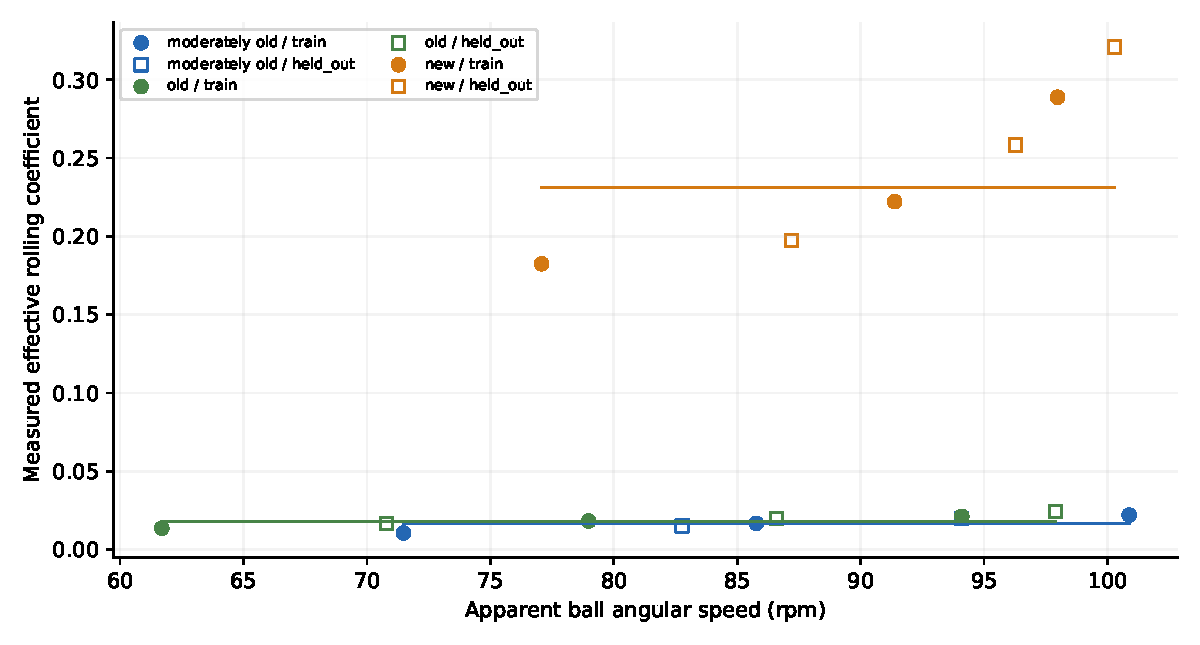
\includegraphics[width=.9\linewidth]{rolling-data.pdf}\end{center}
Circles are calibration points; open squares are held-out points. Horizontal lines
are fitted constants. Each constant improves over an absent rolling moment, but
each loses to the fixed speed-dependent curve. A universal constant is especially
inadequate for the new specimen. This motivates rate-dependent deformation loss,
not an arbitrary per-impact correction.

The source curves were fitted by their authors to these published measurements,
including the points withheld from our constant fit. Their smaller residual is
source reproduction, not independent evidence of predictive superiority. Only the
constant-fit residual has the declared local calibration/test separation.

The apparatus measures quasirolling with slight skid. The estimates are restricted
to the reported apparent-speed ranges and specimens. Ball radii/inertia and complete
matched impact parameters are not supplied. No outgoing bounce state is validated
by these rolling points. One-PDF-point digitization sensitivities and leave-one-out
estimate ranges are retained in the results. Negative source intercepts are not
extrapolated into negative material resistance.

\newpage
\section*{Rocks and non-spherical collision scope}

The 75 limestone/concrete records are genuine experimental magnitudes. The earlier
three-parameter sphere surrogate is recomputed unchanged, with its original
50-record calibration and 25-record release-height holdout. These project estimates
are not independently documented material values. The user now permits small fits,
but this does not make a fitted shape proxy an authentic rock model.
\begin{center}\footnotesize\setlength{\tabcolsep}{4pt}
\begin{tabular}{ll}
\hline
Held-out quantity & RMSE\\\hline
Normal velocity & 1.0044 m/s\\
Tangent velocity & 1.3047 m/s\\
Angular speed & 12.8765 rad/s\\
\hline\end{tabular}\end{center}
Exact collision mesh, central tensor, attitude and signed angular vectors are absent.
Zero incoming spin and coplanar signed reconstruction are assumptions. A conditional
inverse moment is recorded under those same assumptions, but it cannot identify a
true rolling coefficient. All 75 row values remain in the appendix/CSV; failures
are not removed.

The synthetic rotated cuboid, irregular 2D/3D controls and large rapid worlds are
numerical tests. They cannot replace non-spherical experimental validation. The
13-case rapid/irregular baseline remains unqualified. Production still rejects
nonzero rolling/twisting inputs rather than silently accepting an absent mechanism.
The 200 new rolling checks concern a separate sustained-contact branch.

\newpage
\section*{One deviation diagram, with the observations stated}

Each dot compares a predicted outgoing magnitude signature with a measured one.
Horizontal position is the angle between signatures; vertical position is the
relative difference in signature norm. A perfect match is at $(0,0)$. This angle
is not a physical heading error.
\begin{center}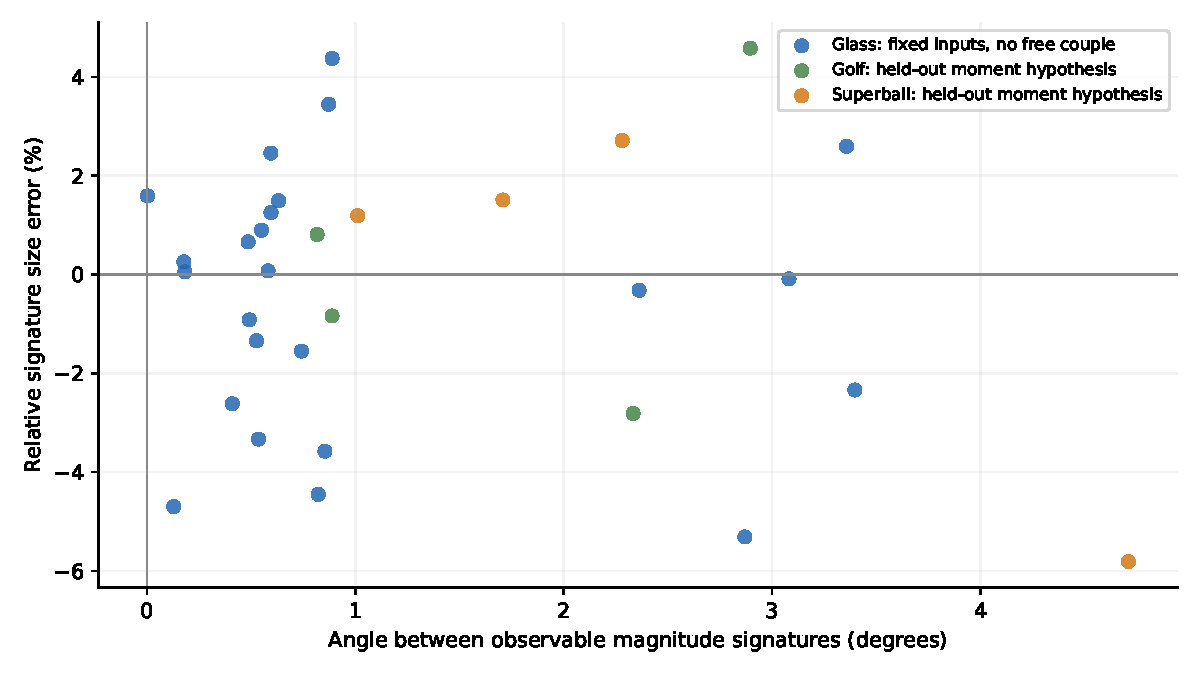
\includegraphics[width=\linewidth]{deviation-map.pdf}\end{center}
Glass uses the two observed translational components. Balls use normal velocity,
tangent velocity and $R|\omega|$; tangent velocity is reconstructed from source
tangential restitution and measured spin. Ball dots use the held-out signed-moment
hypothesis, not same-point exact fits. The signature channels differ, so no pooled
accuracy percentage is computed. Rock dots are excluded from this fresh diagram
because its actual geometry/directional model is not validated.

The standalone HTML plot permits hovering to identify a case. Machine-readable
coordinates, definitions and complete records accompany the PDF. Historical bar
figures are not used as the new model's validation.

\newpage
\section*{Deformation and vibration: the supported next model}

\textbf{Use a finite-duration deformable patch with a small set of internal modes.}
An instantaneous rigid impulse cannot describe the measured stretch, force reversal,
pressure migration and residual vibration. Begin with normal indentation, tangential
shear and a rocking/asymmetric-pressure mode, with positive mass/stiffness and
nonnegative damping. A distributed patch supplies the independent angular impulse:
\[
 \delta\mathbf p=\int\sum_k\mathbf f_k\,dt,\qquad
 \delta\mathbf L=\int\sum_k\rw{\mathbf x_k-\mathbf x_c}\,\mathbf f_k\,dt.
\]
The body's angular update still contains both $\rw{\mathbf r}\,\delta\mathbf p$
and this independent $\delta\mathbf L$. Internal vibration velocities contribute
to each patch point's actual slip. Friction must use that slip, not only an undeformed
rigid contact velocity. The general component map must be checked against those
resultants; silently projecting away an unrepresented moment is unacceptable.

For modal coordinates $\mathbf q$, a compact material model is
\[
 M_q\ddot{\mathbf q}+C_q\dot{\mathbf q}+K_q\mathbf q=H^{\mathsf T}\mathbf f,
 \qquad \mathbf u_c=B\mathbf V+H\dot{\mathbf q}.
\]
Use the gradient of one elastic potential for contact force and moment. Its normal
derivative must be retained if shear stiffness depends on compression. Track rigid
kinetic energy, modal kinetic energy, stored strain and dissipation; do not delete
stored energy when the contact opens. Integrating then yields effective restitution;
do not impose a second endpoint impulse on top of a resolved compliant collision.

Hertz/Mindlin contact and local stick/slip provide an established starting point for
small elastic spheres. Large rubber deformation needs a hyperelastic/viscoelastic
shell or solid description, then modal reduction. Pressure history can produce
rolling resistance; adding a fitted rolling torque to an already resolved loss
mechanism can double-count dissipation. Retain $\mu_r a_r$ only for unresolved loss.

\newpage
\section*{How to select and validate the deformation model}

The Cross 2014 author manuscript contains measured force/spin histories and separate
vibration tests for a hollow ball and a superball. It supports this mechanism, but
its force plate and granite measurements use different counterfaces. Their friction
values must not be mixed. Attached-ball vibration modes also use different boundary
conditions from a free bounce; their frequencies constrain, rather than uniquely
determine, the dynamic contact stiffness. [5]
\begin{center}\footnotesize\setlength{\tabcolsep}{4pt}
\begin{tabular}{llll}
\hline
2014 specimen / pair & Mass & Diameter & Source sliding mu\\\hline
Hollow ball / granite & 44.2 g & 59.4 mm & not reliably measured\\
Solid superball / granite & 46.2 g & 46.0 mm & 0.45 +/- 0.08\\
Hollow ball / G10 force plate & same specimen & same specimen & approximately 1.8\\
\hline\end{tabular}\end{center}
The reported hollow-ball attached-mode periods are approximately 11 ms normal and
5 ms tangential; the solid ball has a 4.5 ms normal period and 3.5 ms high-frequency
tangential period, plus a slower mode. These are separate from the 2010 58 mm
Superball and are not automatically a controlled size-only comparison. Static
friction and modal damping still require independent estimates.

Keep geometry, independently measured modal periods and pair friction fixed where
available. Identify at most a few missing stiffness/damping or patch parameters from
normal force histories and independent vibration decay, then reserve oblique spin
and velocity outputs. Fit a mode's damping from its decay, not from every desired
outgoing spin. Use one parameter set over speed, incidence and incoming spin.

First qualify normal force/time and deformation, then tangential force sign changes,
then the independent moment/angular response. Compare full histories and endpoints,
including worst-case errors, static/sliding transitions and energy. An apparent
endpoint improvement that breaks force histories, restitution inputs or total
passivity is rejected. Test a small patch-resolution ladder and a time-step ladder.
If two or three modes cannot reproduce those independent checks, obtain a converged
finite-element shell/solid reference and reduce its verified modes.

This is a literature-supported implementation direction, not a demonstrated new
data fit. The earlier constant shear/rocking candidate worsened held-out error by
23.7\%; the new shared moment estimate also worsens it. Neither is adopted. Merely
adding another oscillator and tuning it to every endpoint is not sufficient.

Reproduction: run calculate.py into a fresh output directory, run audit.py against
it, render.py, then build.sh. The authoritative evidence is evidence-v3; v1 and v2
are preserved preliminary checkpoints. Source snapshots, SHA-256 values, all records
and the independent audit accompany the report. No generic material lookup can yet
promise authentic full-motion predictions across the requested cases.

\newpage
\section*{Keep rigid bodies: a small contact-memory matrix}

The latest user request favors a contact model that encapsulates local deformation
without deformable meshes for all bodies. Keep the existing rigid-body inertia and
contact mobility. Add elastic history $\boldsymbol\eta$, a small positive stiffness
matrix $K$, and nonnegative damping matrix $C$ at an active contact. Angular history
uses $\ell$ times angular displacement, dual to the angular impulse divided by $\ell$.

For a frozen elastic sticking branch and step $h$, the new research core uses
\begin{align*}
 Z&=\tfrac12h^2K+hC,\\
 [W_d+2Z^{-1}]\boldsymbol\lambda&=-2\mathbf z^- -2Z^{-1}hK\boldsymbol\eta^-,\\
 \mathbf z^+&=\mathbf z^-+W_d\boldsymbol\lambda,\\
 \boldsymbol\eta^+&=\boldsymbol\eta^-+h\mathbf z_m,\qquad
 \mathbf z_m=\tfrac12\mathbf z^-+\tfrac12\mathbf z^+.
\end{align*}
Only a small contact matrix is factored. For constant geometry, step and material
it is cached. Body scatter/gather remains the same impulse update. Linear and
independent angular channels may couple through $K$, while the resulting impulse
components remain $\delta p_n,\delta p_t,\delta L_s/\ell,\delta L_n/\ell$.
The energy balance of this branch is
\[
 \Delta E+\Delta U+h\mathbf z_m^{\mathsf T}C\mathbf z_m=0,\qquad
 U=\tfrac12\boldsymbol\eta^{\mathsf T}K\boldsymbol\eta.
\]
This core is implemented in contact\_memory.py and independently checked with
100 planar and 100 spatial body/contact systems, including 20 dependent-direction
cases. It preserves energy/work and representation-length invariance and shows
second-order convergence to an exact oscillator solution. The physical energy error
is below $1.5\times10^{-15}$ relative in those controls.

Opening, Coulomb yielding, changing directions and nonlinear indentation are not yet
implemented in this new core. It is a verified elastic branch, not a production
collision law or a demonstrated experimental improvement. Contact history cannot
simply be discarded at separation; retained internal vibration or explicit loss
must account for its energy. This is the cheap mechanism to extend, rather than a
per-body deformable mesh.
The current Python four-channel cached step measures 45.4 microseconds median locally. This includes validation and Python overhead; it is not a native end-to-end engine benchmark or an all-case performance guarantee.

\newpage
\section*{Rock friction: pressure and plasticity rather than raw impulse powers}

Indentation, asperity crushing and interlocking can add apparent resistance beyond
a sliding-test coefficient. That possibility does not establish which mechanism
dominates these rock records. Keep documented $\mu_s,\mu_d$ as the underlying pair
coefficients. Model an additional passive deformation/ploughing contribution only
when it is independently constrained. Do not silently call net impulse divided by
normal impulse a measured dynamic coefficient.

A physically scaled candidate variable is maximum indentation relative to local
effective curvature, $\chi=\delta_{\max}/R$. For an elastic Hertz reference with
effective modulus $E^*$, coefficient $k_H=4E^*\sqrt R/3$ and incident normal energy
$E_n$, the estimated compression is
\[
 U_n=\tfrac25 k_H\delta^{5/2},\qquad
 \delta_{\max}=\left[\frac{5E_n}{2k_H}\right]^{2/5}.
\]
This is a local proxy valid for small elastic contact, not a solution for crushing
angular rock facets. A yield/history variable is needed once that approximation
breaks down. Thornton--Ning provides an established elastic/plastic normal-contact
route; LAMMPS granular contact demonstrates practical normal, shear-history,
rolling and torsion laws with rigid particles. [10,11]

An $a\chi+b\chi^2$ correction can be tested as a bounded approximation to extra
resistance or a moment-length response over a declared range. It is a hypothesis,
not a proven material law. Fit at most one or two missing coefficients to a training
condition, hold material friction fixed, and reject it if held-out velocity/spin,
worst-case error or passivity worsens. Check identifiability against contact size,
yield and initial-spin uncertainty.

Unnormalized impulse-polynomial coefficients have units and can change meaning
with mass, size and the interval over which impulse is accumulated. For a resting
contact that interval changes with timestep. If an impulse variable is used, it must
refer to the complete impact and an independently specified physical impulse scale,
not the arbitrary coordinate length $\ell$. Pressure, contact work or $\chi$ offer
a clearer route to transferring coefficients across sizes. No pressure-dependent
rock law has been adopted or fitted in the reported comparisons.

\newpage
\section*{Primary sources and current limitations}
[1] \href{https://grainflowresearch.mae.cornell.edu/impact/data/Impact%20Results.html}{Cornell impact coefficients}

[2] \href{https://grainflowresearch.mae.cornell.edu/impact/data/Results-3mmglass-binary}{Original glass worksheet}

[3] \href{https://www.physics.usyd.edu.au/~cross/PUBLICATIONS/48.%20EnhanceBounce.pdf}{Cross 2010: ball/surface experiments}

[4] \href{https://doi.org/10.5194/nhess-18-3045-2018}{Wang et al. 2018: rock impacts}

[5] \href{https://www.researchgate.net/publication/278104773_Oblique_Bounce_of_a_Rubber_Ball}{Cross 2014: oblique rubber bounce, author manuscript}

[6] \href{https://arxiv.org/abs/0809.4823}{Singh et al. 2008: rolling experiment}

[7] \href{https://www2.msm.ctw.utwente.nl/sluding/PAPERS/2014_WeinhartFuchs_GMr.pdf}{Fuchs et al. 2014: rolling/sliding/torsion}

[8] \href{https://websites.umich.edu/~jbarber/Wear1976.pdf}{Maw, Barber and Fawcett 1976: elastic oblique contact}

[9] \href{https://ntrs.nasa.gov/api/citations/20050217091/downloads/20050217091.pdf}{NASA 2005: measured rolling and failed bounce extension}

[10] \href{https://docs.lammps.org/pair_granular.html}{LAMMPS granular contact: history, rolling and torsion}

[11] \href{https://doi.org/10.1016/S0032-5910(98)00099-0}{Thornton--Ning 1998: elastic/plastic normal contact}

Full measured signed 3D states and central tensors are not available for the
recovered rock fixtures. Dynamic/static/rolling profiles remain incomplete for
most pairs. Published coefficient charts, worksheet reconstructions and singleton
summary rows cannot independently identify every angular/material channel. Those
limits constrain what the present numbers establish; they are not hidden defaults.

\newpage
\section*{Appendix: all 24 glass collision comparisons}
\begin{center}\footnotesize\setlength{\tabcolsep}{4pt}
\begin{tabular}{lllll}
\hline
Excel row & Normal obs. & Normal pred. & Tangent obs. & Tangent pred.\\\hline
2 & 0.92521 & 0.97668 & -0.48443 & -0.44054\\
13 & 0.86685 & 0.80824 & -0.63661 & -0.67081\\
24 & 0.74446 & 0.73741 & -0.74531 & -0.75337\\
35 & 0.85223 & 0.89104 & -0.60724 & -0.61467\\
46 & 0.56947 & 0.61812 & -0.93034 & -0.89759\\
57 & 0.69712 & 0.69487 & -0.78925 & -0.77232\\
68 & 1.02769 & 0.95319 & -0.39398 & -0.42130\\
79 & 0.91821 & 0.92967 & -0.63660 & -0.63296\\
90 & 0.99824 & 0.98450 & -0.53381 & -0.53736\\
101 & 0.96391 & 0.93751 & -0.54760 & -0.58497\\
112 & 1.07357 & 1.02150 & -0.30496 & -0.30607\\
123 & 1.14587 & 1.19960 & -0.23465 & -0.22634\\
134 & 1.12873 & 1.14806 & -0.22810 & -0.21887\\
145 & 1.16067 & 1.17914 & -0.22808 & -0.23167\\
156 & 1.17884 & 1.19401 & -0.04548 & -0.03366\\
167 & 1.21576 & 1.15873 & -0.04107 & -0.03655\\
178 & 1.13198 & 1.16148 & -0.16552 & -0.15756\\
189 & 1.16999 & 1.12545 & 0.17683 & 0.18729\\
200 & 1.18091 & 1.19323 & 0.18636 & 0.17660\\
211 & 1.12379 & 1.08438 & 0.21220 & 0.21526\\
222 & 1.21562 & 1.21592 & 0.11036 & 0.11427\\
233 & 1.25086 & 1.23072 & 0.04908 & 0.06424\\
244 & 1.10217 & 1.07165 & 0.23806 & 0.23948\\
255 & 1.16525 & 1.16854 & 0.10528 & 0.10196\\
\hline\end{tabular}\end{center}All values are m/s. Tangent output is the source-reconstructed COM quantity. No independently measured spin is added.
\newpage
\section*{Appendix: rock records 1--25}
\begin{center}\footnotesize\setlength{\tabcolsep}{4pt}
\begin{tabular}{lllll}
\hline
Row & Split & v\_n obs/pred & v\_t obs/pred & omega obs/pred\\\hline
18 & train & 2.570 / 2.645 & 2.898 / 2.807 & 48.40 / 42.15\\
19 & train & 1.714 / 2.836 & 2.824 / 2.610 & 43.20 / 39.20\\
20 & train & 1.929 / 2.612 & 2.902 / 2.718 & 41.50 / 40.83\\
21 & train & 2.826 / 2.684 & 2.655 / 2.673 & 49.20 / 40.14\\
22 & train & 2.536 / 3.231 & 3.342 / 3.154 & 50.60 / 47.36\\
23 & train & 2.683 / 3.113 & 4.008 / 3.376 & 55.40 / 50.70\\
24 & train & 2.184 / 3.293 & 4.168 / 3.152 & 44.80 / 47.34\\
25 & test & 3.039 / 3.821 & 3.947 / 3.465 & 51.30 / 52.04\\
26 & test & 3.177 / 3.676 & 4.074 / 3.784 & 65.80 / 56.83\\
27 & test & 2.718 / 3.895 & 4.537 / 3.740 & 59.20 / 56.16\\
28 & train & 2.141 / 1.968 & 3.879 / 3.621 & 42.60 / 54.37\\
29 & train & 2.562 / 2.087 & 3.852 / 3.944 & 53.70 / 59.23\\
30 & train & 2.040 / 2.033 & 4.628 / 3.715 & 39.80 / 55.79\\
31 & train & 1.952 / 1.930 & 3.739 / 3.944 & 46.40 / 59.22\\
32 & train & 2.723 / 2.440 & 4.468 / 4.545 & 58.00 / 68.25\\
33 & train & 2.406 / 2.360 & 5.258 / 4.559 & 53.20 / 68.46\\
34 & train & 2.403 / 2.397 & 4.248 / 4.727 & 51.60 / 70.99\\
35 & test & 2.696 / 2.757 & 4.682 / 5.122 & 67.60 / 76.92\\
36 & test & 3.722 / 2.809 & 4.509 / 5.262 & 58.20 / 79.03\\
37 & test & 3.342 / 2.723 & 5.349 / 5.148 & 54.10 / 77.31\\
38 & train & 2.074 / 1.242 & 3.755 / 4.450 & 66.80 / 66.82\\
39 & train & 2.230 / 1.414 & 4.220 / 4.427 & 59.40 / 66.49\\
40 & train & 1.951 / 1.426 & 4.234 / 4.733 & 61.70 / 71.07\\
41 & train & 2.797 / 1.667 & 6.323 / 5.680 & 62.40 / 85.30\\
42 & train & 2.713 / 1.708 & 4.828 / 5.500 & 81.30 / 82.60\\
\hline\end{tabular}\end{center}Velocities are m/s; angular speed is rad/s. Prediction is the historical sphere proxy, not actual rock geometry. ``test denotes the original release-height holdout.
\newpage
\section*{Appendix: rock records 26--50}
\begin{center}\footnotesize\setlength{\tabcolsep}{4pt}
\begin{tabular}{lllll}
\hline
Row & Split & v\_n obs/pred & v\_t obs/pred & omega obs/pred\\\hline
43 & train & 3.613 / 1.722 & 3.849 / 5.314 & 75.40 / 79.80\\
44 & test & 2.016 / 2.161 & 5.663 / 6.023 & 64.30 / 90.45\\
45 & test & 2.913 / 1.878 & 5.374 / 6.150 & 81.50 / 92.36\\
46 & test & 1.414 / 1.872 & 5.394 / 5.917 & 66.20 / 88.86\\
47 & train & 1.582 / 0.676 & 3.192 / 5.040 & 75.90 / 75.69\\
48 & train & 1.553 / 0.814 & 3.378 / 4.680 & 68.20 / 70.29\\
49 & train & 1.158 / 0.623 & 3.367 / 4.839 & 73.10 / 72.68\\
50 & train & 1.641 / 0.705 & 4.421 / 5.941 & 91.20 / 86.69\\
51 & train & 1.110 / 0.722 & 7.117 / 6.056 & 53.50 / 88.68\\
52 & train & 1.786 / 0.616 & 3.551 / 6.359 & 85.60 / 75.72\\
53 & test & 1.663 / 0.641 & 5.281 / 7.182 & 97.50 / 78.81\\
54 & test & 3.054 / 0.757 & 3.924 / 7.353 & 107.20 / 92.99\\
55 & test & 3.176 / 0.891 & 4.014 / 6.905 & 93.20 / 103.70\\
57 & train & 2.119 / 2.645 & 2.728 / 2.507 & 20.60 / 18.82\\
58 & train & 2.337 / 2.789 & 3.326 / 2.830 & 19.70 / 21.25\\
59 & train & 2.073 / 2.647 & 3.030 / 2.642 & 24.80 / 19.84\\
60 & train & 2.289 / 3.233 & 3.281 / 3.169 & 29.20 / 23.80\\
61 & train & 1.908 / 3.396 & 4.134 / 3.063 & 23.00 / 23.00\\
62 & train & 1.911 / 3.162 & 3.510 / 3.268 & 27.90 / 24.54\\
63 & test & 2.833 / 3.627 & 4.664 / 3.924 & 30.40 / 29.46\\
64 & test & 3.058 / 3.722 & 3.853 / 3.540 & 31.60 / 26.58\\
65 & test & 2.356 / 3.663 & 3.725 / 3.362 & 25.80 / 25.25\\
66 & test & 2.869 / 3.854 & 3.728 / 3.661 & 26.30 / 27.49\\
67 & train & 2.769 / 2.272 & 3.596 / 3.682 & 33.80 / 27.65\\
68 & train & 2.334 / 2.052 & 3.156 / 3.508 & 27.40 / 26.34\\
\hline\end{tabular}\end{center}Velocities are m/s; angular speed is rad/s. Prediction is the historical sphere proxy, not actual rock geometry. ``test denotes the original release-height holdout.
\newpage
\section*{Appendix: rock records 51--75}
\begin{center}\footnotesize\setlength{\tabcolsep}{4pt}
\begin{tabular}{lllll}
\hline
Row & Split & v\_n obs/pred & v\_t obs/pred & omega obs/pred\\\hline
69 & train & 2.028 / 1.933 & 3.880 / 4.060 & 32.10 / 30.48\\
70 & train & 2.883 / 2.503 & 4.313 / 4.732 & 37.60 / 35.53\\
71 & train & 2.365 / 2.650 & 3.879 / 4.566 & 28.70 / 34.29\\
72 & train & 2.295 / 2.421 & 4.609 / 4.751 & 31.50 / 35.67\\
73 & test & 2.337 / 2.818 & 5.436 / 5.180 & 29.40 / 38.90\\
74 & test & 3.239 / 2.704 & 5.645 / 5.054 & 29.70 / 37.95\\
75 & test & 2.337 / 2.818 & 6.109 / 5.180 & 22.70 / 38.90\\
76 & train & 2.097 / 1.244 & 4.176 / 4.411 & 39.40 / 33.12\\
77 & train & 2.517 / 1.543 & 4.035 / 4.233 & 32.60 / 31.79\\
78 & train & 1.900 / 1.424 & 3.927 / 4.377 & 31.50 / 32.86\\
79 & train & 1.909 / 1.525 & 5.111 / 5.213 & 31.70 / 39.14\\
80 & train & 2.208 / 1.624 & 4.100 / 5.325 & 38.40 / 39.99\\
81 & train & 2.958 / 1.575 & 4.362 / 5.292 & 42.50 / 39.73\\
82 & test & 2.767 / 1.875 & 3.963 / 6.156 & 40.20 / 46.22\\
83 & test & 1.944 / 2.041 & 5.291 / 6.072 & 31.30 / 45.59\\
84 & test & 3.036 / 2.045 & 5.309 / 5.702 & 45.30 / 42.81\\
85 & train & 1.239 / 0.699 & 3.645 / 4.529 & 40.50 / 34.01\\
86 & train & 0.893 / 0.561 & 4.109 / 4.810 & 37.60 / 34.47\\
87 & train & 0.743 / 0.516 & 4.885 / 4.541 & 25.20 / 31.71\\
88 & train & 1.423 / 0.618 & 5.650 / 5.323 & 32.80 / 37.95\\
89 & train & 1.439 / 0.895 & 4.719 / 5.425 & 31.60 / 40.73\\
90 & train & 1.709 / 0.647 & 4.014 / 5.956 & 42.00 / 39.77\\
91 & test & 1.993 / 0.962 & 4.991 / 6.141 & 43.90 / 46.11\\
92 & test & 1.617 / 0.742 & 6.100 / 5.735 & 35.60 / 43.07\\
93 & test & 1.357 / 0.468 & 4.224 / 6.865 & 45.00 / 28.77\\
\hline\end{tabular}\end{center}Velocities are m/s; angular speed is rad/s. Prediction is the historical sphere proxy, not actual rock geometry. ``test denotes the original release-height holdout.
\newpage
\section*{Appendix: all 17 digitized rolling measurements}
\begin{center}\footnotesize\setlength{\tabcolsep}{4pt}
\begin{tabular}{llllll}
\hline
Specimen & Split & rpm & Measured mu\_r & Constant & Fixed curve\\\hline
moderately\_old & train & 71.483 & 0.010602 & 0.016438 & 0.011023\\
moderately\_old & held\_out & 82.770 & 0.015113 & 0.016438 & 0.015763\\
moderately\_old & train & 85.771 & 0.016700 & 0.016438 & 0.017024\\
moderately\_old & held\_out & 94.088 & 0.019708 & 0.016438 & 0.020517\\
moderately\_old & train & 100.872 & 0.022013 & 0.016438 & 0.023366\\
old & train & 61.694 & 0.013609 & 0.017675 & 0.013740\\
old & held\_out & 70.795 & 0.016700 & 0.017675 & 0.016107\\
old & train & 78.984 & 0.018204 & 0.017675 & 0.018236\\
old & held\_out & 86.583 & 0.019708 & 0.017675 & 0.020212\\
old & train & 94.094 & 0.021211 & 0.017675 & 0.022164\\
old & held\_out & 97.894 & 0.024302 & 0.017675 & 0.023152\\
new & train & 77.077 & 0.182403 & 0.231073 & 0.167046\\
new & held\_out & 87.189 & 0.197341 & 0.231073 & 0.225697\\
new & train & 91.376 & 0.222060 & 0.231073 & 0.249979\\
new & held\_out & 96.272 & 0.258371 & 0.231073 & 0.278380\\
new & train & 97.975 & 0.288755 & 0.231073 & 0.288257\\
new & held\_out & 100.282 & 0.320945 & 0.231073 & 0.301633\\
\hline\end{tabular}\end{center}
\end{document}
